\documentclass[twoside]{book}

% Packages required by doxygen
\usepackage{fixltx2e}
\usepackage{calc}
\usepackage{doxygen}
\usepackage[export]{adjustbox} % also loads graphicx
\usepackage{graphicx}
\usepackage[utf8]{inputenc}
\usepackage{makeidx}
\usepackage{multicol}
\usepackage{multirow}
\PassOptionsToPackage{warn}{textcomp}
\usepackage{textcomp}
\usepackage[nointegrals]{wasysym}
\usepackage[table]{xcolor}

% Font selection
\usepackage[T1]{fontenc}
\usepackage[scaled=.90]{helvet}
\usepackage{courier}
\usepackage{amssymb}
\usepackage{sectsty}
\renewcommand{\familydefault}{\sfdefault}
\allsectionsfont{%
  \fontseries{bc}\selectfont%
  \color{darkgray}%
}
\renewcommand{\DoxyLabelFont}{%
  \fontseries{bc}\selectfont%
  \color{darkgray}%
}
\newcommand{\+}{\discretionary{\mbox{\scriptsize$\hookleftarrow$}}{}{}}

% Page & text layout
\usepackage{geometry}
\geometry{%
  a4paper,%
  top=2.5cm,%
  bottom=2.5cm,%
  left=2.5cm,%
  right=2.5cm%
}
\tolerance=750
\hfuzz=15pt
\hbadness=750
\setlength{\emergencystretch}{15pt}
\setlength{\parindent}{0cm}
\setlength{\parskip}{0.2cm}
\makeatletter
\renewcommand{\paragraph}{%
  \@startsection{paragraph}{4}{0ex}{-1.0ex}{1.0ex}{%
    \normalfont\normalsize\bfseries\SS@parafont%
  }%
}
\renewcommand{\subparagraph}{%
  \@startsection{subparagraph}{5}{0ex}{-1.0ex}{1.0ex}{%
    \normalfont\normalsize\bfseries\SS@subparafont%
  }%
}
\makeatother

% Headers & footers
\usepackage{fancyhdr}
\pagestyle{fancyplain}
\fancyhead[LE]{\fancyplain{}{\bfseries\thepage}}
\fancyhead[CE]{\fancyplain{}{}}
\fancyhead[RE]{\fancyplain{}{\bfseries\leftmark}}
\fancyhead[LO]{\fancyplain{}{\bfseries\rightmark}}
\fancyhead[CO]{\fancyplain{}{}}
\fancyhead[RO]{\fancyplain{}{\bfseries\thepage}}
\fancyfoot[LE]{\fancyplain{}{}}
\fancyfoot[CE]{\fancyplain{}{}}
\fancyfoot[RE]{\fancyplain{}{\bfseries\scriptsize Generated on Wed Apr 22 2015 12\+:12\+:47 for M\+R\+D\+B\+C by Doxygen }}
\fancyfoot[LO]{\fancyplain{}{\bfseries\scriptsize Generated on Wed Apr 22 2015 12\+:12\+:47 for M\+R\+D\+B\+C by Doxygen }}
\fancyfoot[CO]{\fancyplain{}{}}
\fancyfoot[RO]{\fancyplain{}{}}
\renewcommand{\footrulewidth}{0.4pt}
\renewcommand{\chaptermark}[1]{%
  \markboth{#1}{}%
}
\renewcommand{\sectionmark}[1]{%
  \markright{\thesection\ #1}%
}

% Indices & bibliography
\usepackage{natbib}
\usepackage[titles]{tocloft}
\setcounter{tocdepth}{3}
\setcounter{secnumdepth}{5}
\makeindex

% Hyperlinks (required, but should be loaded last)
\usepackage{ifpdf}
\ifpdf
  \usepackage[pdftex,pagebackref=true]{hyperref}
\else
  \usepackage[ps2pdf,pagebackref=true]{hyperref}
\fi
\hypersetup{%
  colorlinks=true,%
  linkcolor=blue,%
  citecolor=blue,%
  unicode%
}

% Custom commands
\newcommand{\clearemptydoublepage}{%
  \newpage{\pagestyle{empty}\cleardoublepage}%
}


%===== C O N T E N T S =====

\begin{document}

% Titlepage & ToC
\hypersetup{pageanchor=false,
             bookmarks=true,
             bookmarksnumbered=true,
             pdfencoding=unicode
            }
\pagenumbering{roman}
\begin{titlepage}
\vspace*{7cm}
\begin{center}%
{\Large M\+R\+D\+B\+C \\[1ex]\large 0.\+1 }\\
\vspace*{1cm}
{\large Generated by Doxygen 1.8.9.1}\\
\vspace*{0.5cm}
{\small Wed Apr 22 2015 12:12:47}\\
\end{center}
\end{titlepage}
\clearemptydoublepage
\tableofcontents
\clearemptydoublepage
\pagenumbering{arabic}
\hypersetup{pageanchor=true}

%--- Begin generated contents ---
\chapter{C\+U\+D\+A\+D\+Clusterer}
\label{md_README}
\hypertarget{md_README}{}
A fast implementation of the density cluster algorithm in C\+U\+D\+A of biological datasets.

C\+U\+D\+A\+D\+Clusterer uses the .xtc Groomacs file extension.

\subsection*{Requirements }


\begin{DoxyItemize}
\item C\+Make 3.\+2.\+1
\item G\+C\+C 4.\+9.\+2
\item C\+U\+D\+A 7.\+0
\item Boost 1.\+57
\end{DoxyItemize}

{\bfseries O\+B\+S\+:} These requirements were tested and proved to work. Feel free to test older versions of the requirements

\subsection*{T\+O\+D\+O }


\begin{DoxyItemize}
\item \mbox{[}x\mbox{]} .xtc file parser \mbox{[}I\+M\+P\mbox{]}
\item \mbox{[} \mbox{]} C\+U\+D\+A clusterer kernel
\item \mbox{[} \mbox{]} Dimentionality reduction
\item \mbox{[} \mbox{]} Data Visualizer
\end{DoxyItemize}

labels\+:
\begin{DoxyItemize}
\item \mbox{[}D\+O\+N\mbox{]} -\/ Done
\item \mbox{[}I\+M\+P\mbox{]} -\/ To be improoved
\item \mbox{[}B\+U\+G\mbox{]} -\/ Buggy and experimental
\end{DoxyItemize}

\subsection*{Credits }

{\bfseries Author\+:} \href{https://github.com/tlgimenes}{\tt Tiago L\+O\+B\+A\+T\+O G\+I\+M\+E\+N\+E\+S}\+: $\ast$tlgimenes.com$\ast$

{\bfseries Contributors\+:} Maybe you ! 
\chapter{Hierarchical Index}
\section{Class Hierarchy}
This inheritance list is sorted roughly, but not completely, alphabetically\+:\begin{DoxyCompactList}
\item \contentsline{section}{adjacency\+\_\+graph}{\pageref{classadjacency__graph}}{}
\item \contentsline{section}{cluster\+:\+:dbscan}{\pageref{classcluster_1_1dbscan}}{}
\begin{DoxyCompactList}
\item \contentsline{section}{cluster\+:\+:cpu\+:\+:dbscan}{\pageref{classcluster_1_1cpu_1_1dbscan}}{}
\end{DoxyCompactList}
\item \contentsline{section}{key\+\_\+value$<$ K, V $>$}{\pageref{classkey__value}}{}
\item \contentsline{section}{console\+:\+:modifier}{\pageref{classconsole_1_1modifier}}{}
\item \contentsline{section}{console\+:\+:parser}{\pageref{classconsole_1_1parser}}{}
\item \contentsline{section}{primitive$<$ T, N $>$}{\pageref{classprimitive}}{}
\item \contentsline{section}{reader\+\_\+xtc}{\pageref{classreader__xtc}}{}
\item \contentsline{section}{tree\+:\+:vp\+\_\+node\+\_\+t}{\pageref{structtree_1_1vp__node__t}}{}
\item \contentsline{section}{tree\+:\+:vp\+\_\+tree}{\pageref{classtree_1_1vp__tree}}{}
\begin{DoxyCompactList}
\item \contentsline{section}{tree\+:\+:cpu\+:\+:vp\+\_\+tree}{\pageref{classtree_1_1cpu_1_1vp__tree}}{}
\end{DoxyCompactList}
\end{DoxyCompactList}

\chapter{Class Index}
\section{Class List}
Here are the classes, structs, unions and interfaces with brief descriptions\+:\begin{DoxyCompactList}
\item\contentsline{section}{\hyperlink{classadjacency__graph}{adjacency\+\_\+graph} }{\pageref{classadjacency__graph}}{}
\item\contentsline{section}{\hyperlink{classcluster_1_1cpu_1_1dbscan}{cluster\+::cpu\+::dbscan} \\*Class for applying D\+B\+S\+C\+A\+N clustering algorithm to data }{\pageref{classcluster_1_1cpu_1_1dbscan}}{}
\item\contentsline{section}{\hyperlink{classcluster_1_1dbscan}{cluster\+::dbscan} \\*Base class for applying D\+B\+S\+C\+A\+N clustering algorithm to data }{\pageref{classcluster_1_1dbscan}}{}
\item\contentsline{section}{\hyperlink{classkey__value}{key\+\_\+value$<$ K, V $>$} \\*Key-\/\+Value class implementation }{\pageref{classkey__value}}{}
\item\contentsline{section}{\hyperlink{classconsole_1_1modifier}{console\+::modifier} }{\pageref{classconsole_1_1modifier}}{}
\item\contentsline{section}{\hyperlink{classconsole_1_1parser}{console\+::parser} \\*Class for parsing the Command Line Interface }{\pageref{classconsole_1_1parser}}{}
\item\contentsline{section}{\hyperlink{classprimitive}{primitive$<$ T, N $>$} \\*Implementation of general N-\/dimentional type }{\pageref{classprimitive}}{}
\item\contentsline{section}{\hyperlink{classreader__xtc}{reader\+\_\+xtc} \\*Class for reading trajlist and .xtc files }{\pageref{classreader__xtc}}{}
\item\contentsline{section}{\hyperlink{structtree_1_1vp__node__t}{tree\+::vp\+\_\+node\+\_\+t} \\*Vp-\/tree node for a linearized tree in an array }{\pageref{structtree_1_1vp__node__t}}{}
\item\contentsline{section}{\hyperlink{classtree_1_1vp__tree}{tree\+::vp\+\_\+tree} \\*Base class for creating vp-\/tree }{\pageref{classtree_1_1vp__tree}}{}
\item\contentsline{section}{\hyperlink{classtree_1_1cpu_1_1vp__tree}{tree\+::cpu\+::vp\+\_\+tree} \\*Base class for creating vp-\/tree }{\pageref{classtree_1_1cpu_1_1vp__tree}}{}
\end{DoxyCompactList}

\chapter{Class Documentation}
\hypertarget{classAdjacencyGraph}{}\section{Adjacency\+Graph Class Reference}
\label{classAdjacencyGraph}\index{Adjacency\+Graph@{Adjacency\+Graph}}


The documentation for this class was generated from the following file\+:\begin{DoxyCompactItemize}
\item 
knn/adjacency\+\_\+graph.\+hpp\end{DoxyCompactItemize}

\hypertarget{classDBSCAN}{}\section{D\+B\+S\+C\+A\+N Class Reference}
\label{classDBSCAN}\index{D\+B\+S\+C\+A\+N@{D\+B\+S\+C\+A\+N}}
\subsection*{Public Member Functions}
\begin{DoxyCompactItemize}
\item 
\hypertarget{classDBSCAN_aa4de8fb630dbe6c15042c2283e7b4a60}{}{\bfseries D\+B\+S\+C\+A\+N} (const std\+::vector$<$ float $>$ \&\+\_\+data, const float \hyperlink{classDBSCAN_a3b455b232e38ffebc80e81782b78abbf}{eps}, const int min\+\_\+pts, const int dim)\label{classDBSCAN_aa4de8fb630dbe6c15042c2283e7b4a60}

\item 
float \& \hyperlink{classDBSCAN_a3b455b232e38ffebc80e81782b78abbf}{eps} ()
\item 
\hypertarget{classDBSCAN_a96999b24db2fb5a2731935190b727a42}{}float \& {\bfseries min\+\_\+pts} ()\label{classDBSCAN_a96999b24db2fb5a2731935190b727a42}

\item 
const float \& \hyperlink{classDBSCAN_a38e394f6c2be17c39a21f403d17932f9}{eps} () const 
\item 
\hypertarget{classDBSCAN_a41e51384471a32fcd59f7229a7979cf1}{}const float \& {\bfseries min\+\_\+pts} () const \label{classDBSCAN_a41e51384471a32fcd59f7229a7979cf1}

\end{DoxyCompactItemize}
\subsection*{Protected Attributes}
\begin{DoxyCompactItemize}
\item 
\hypertarget{classDBSCAN_a509e3960831c976805b9c83ebcd82735}{}float {\bfseries \+\_\+eps}\label{classDBSCAN_a509e3960831c976805b9c83ebcd82735}

\item 
\hypertarget{classDBSCAN_a62a7932b88a1d4311b533efa38c9700b}{}int {\bfseries \+\_\+min\+\_\+pts}\label{classDBSCAN_a62a7932b88a1d4311b533efa38c9700b}

\item 
\hypertarget{classDBSCAN_a3ca40201957cf715a727b039983d5e6d}{}int {\bfseries \+\_\+dim}\label{classDBSCAN_a3ca40201957cf715a727b039983d5e6d}

\item 
\hypertarget{classDBSCAN_ac1b6e7c55ca50a540339dbf803969d06}{}const std\+::vector$<$ float $>$ \& {\bfseries \+\_\+data}\label{classDBSCAN_ac1b6e7c55ca50a540339dbf803969d06}

\end{DoxyCompactItemize}


\subsection{Member Function Documentation}
\hypertarget{classDBSCAN_a3b455b232e38ffebc80e81782b78abbf}{}\index{D\+B\+S\+C\+A\+N@{D\+B\+S\+C\+A\+N}!eps@{eps}}
\index{eps@{eps}!D\+B\+S\+C\+A\+N@{D\+B\+S\+C\+A\+N}}
\subsubsection[{eps}]{\setlength{\rightskip}{0pt plus 5cm}float\& D\+B\+S\+C\+A\+N\+::eps (
\begin{DoxyParamCaption}
{}
\end{DoxyParamCaption}
)\hspace{0.3cm}{\ttfamily [inline]}}\label{classDBSCAN_a3b455b232e38ffebc80e81782b78abbf}
Sets \hypertarget{classDBSCAN_a38e394f6c2be17c39a21f403d17932f9}{}\index{D\+B\+S\+C\+A\+N@{D\+B\+S\+C\+A\+N}!eps@{eps}}
\index{eps@{eps}!D\+B\+S\+C\+A\+N@{D\+B\+S\+C\+A\+N}}
\subsubsection[{eps}]{\setlength{\rightskip}{0pt plus 5cm}const float\& D\+B\+S\+C\+A\+N\+::eps (
\begin{DoxyParamCaption}
{}
\end{DoxyParamCaption}
) const\hspace{0.3cm}{\ttfamily [inline]}}\label{classDBSCAN_a38e394f6c2be17c39a21f403d17932f9}
Gets 

The documentation for this class was generated from the following file\+:\begin{DoxyCompactItemize}
\item 
clusterer/dbscan.\+hpp\end{DoxyCompactItemize}

\hypertarget{classifloatn}{}\section{ifloatn$<$ N $>$ Class Template Reference}
\label{classifloatn}\index{ifloatn$<$ N $>$@{ifloatn$<$ N $>$}}
\subsection*{Public Member Functions}
\begin{DoxyCompactItemize}
\item 
\hypertarget{classifloatn_ae28a7ea70c26043ded183cd8c85e4add}{}{\bfseries ifloatn} (const \hyperlink{classprimitive}{floatn}$<$ N $>$ \&v, const \hyperlink{classprimitive}{intn}$<$ N $>$ \&k)\label{classifloatn_ae28a7ea70c26043ded183cd8c85e4add}

\item 
\hypertarget{classifloatn_a5f04e357bb5d2862bfc81c4e80cdc448}{}const \hyperlink{classprimitive}{floatn}$<$ N $>$ \& {\bfseries val} () const \label{classifloatn_a5f04e357bb5d2862bfc81c4e80cdc448}

\item 
\hypertarget{classifloatn_ad9105e98e1a72be41a1a1eb98ff20b06}{}const \hyperlink{classprimitive}{intn}$<$ N $>$ \& {\bfseries key} () const \label{classifloatn_ad9105e98e1a72be41a1a1eb98ff20b06}

\item 
\hypertarget{classifloatn_a3e1052ebea54413dc5eb48da500741e4}{}\hyperlink{classprimitive}{floatn}$<$ N $>$ \& {\bfseries val} ()\label{classifloatn_a3e1052ebea54413dc5eb48da500741e4}

\item 
\hypertarget{classifloatn_aad1c244555efb5e6e0809af69321797f}{}\hyperlink{classprimitive}{intn}$<$ N $>$ \& {\bfseries key} ()\label{classifloatn_aad1c244555efb5e6e0809af69321797f}

\item 
\hypertarget{classifloatn_a083935b6c13dbcdd3a962fab73ff91b1}{}const \hyperlink{classifloatn}{ifloatn}$<$ N $>$ \& {\bfseries operator=} (const \hyperlink{classifloatn}{ifloatn}$<$ N $>$ \&other)\label{classifloatn_a083935b6c13dbcdd3a962fab73ff91b1}

\item 
\hypertarget{classifloatn_a7970284682bb83be713e03bef0fbc1cf}{}bool {\bfseries operator$<$} (const \hyperlink{classifloatn}{ifloatn} \&i) const \label{classifloatn_a7970284682bb83be713e03bef0fbc1cf}

\end{DoxyCompactItemize}
\subsection*{Protected Attributes}
\begin{DoxyCompactItemize}
\item 
\hypertarget{classifloatn_aaeda646e8023f9b0ceb60a4ecdbe5010}{}\hyperlink{classprimitive}{floatn}$<$ N $>$ {\bfseries \+\_\+val}\label{classifloatn_aaeda646e8023f9b0ceb60a4ecdbe5010}

\item 
\hypertarget{classifloatn_aac28a60f55fcdf647c049d2511a67690}{}\hyperlink{classprimitive}{intn}$<$ N $>$ {\bfseries \+\_\+key}\label{classifloatn_aac28a60f55fcdf647c049d2511a67690}

\end{DoxyCompactItemize}


The documentation for this class was generated from the following file\+:\begin{DoxyCompactItemize}
\item 
utils/types.\+hpp\end{DoxyCompactItemize}

\hypertarget{classParser}{}\section{Parser Class Reference}
\label{classParser}\index{Parser@{Parser}}
\subsection*{Static Public Member Functions}
\begin{DoxyCompactItemize}
\item 
static void \hyperlink{classParser_a1974bdd5c298fa16b72abfbc6b857e7d}{parse} (int argc, const char $\ast$$\ast$argv)
\item 
static void \hyperlink{classParser_ac335c7e97598e58fae32e8449e6f3f39}{add\+\_\+argument} (const std\+::string \&short\+\_\+form, const std\+::string \&help)
\item 
static const std\+::string \hyperlink{classParser_a2e974f6de03f79aeac39eba63afd6f1e}{get} (const std\+::string \&arg, bool required)
\end{DoxyCompactItemize}
\subsection*{Static Protected Member Functions}
\begin{DoxyCompactItemize}
\item 
static void \hyperlink{classParser_ab7e0b95b8d8904a0bdeae8721fdee749}{print\+\_\+help} ()
\end{DoxyCompactItemize}


\subsection{Member Function Documentation}
\hypertarget{classParser_ac335c7e97598e58fae32e8449e6f3f39}{}\index{Parser@{Parser}!add\+\_\+argument@{add\+\_\+argument}}
\index{add\+\_\+argument@{add\+\_\+argument}!Parser@{Parser}}
\subsubsection[{add\+\_\+argument}]{\setlength{\rightskip}{0pt plus 5cm}void Parser\+::add\+\_\+argument (
\begin{DoxyParamCaption}
\item[{const std\+::string \&}]{short\+\_\+form, }
\item[{const std\+::string \&}]{help}
\end{DoxyParamCaption}
)\hspace{0.3cm}{\ttfamily [inline]}, {\ttfamily [static]}}\label{classParser_ac335c7e97598e58fae32e8449e6f3f39}
Adds arguments to be parsed \hypertarget{classParser_a2e974f6de03f79aeac39eba63afd6f1e}{}\index{Parser@{Parser}!get@{get}}
\index{get@{get}!Parser@{Parser}}
\subsubsection[{get}]{\setlength{\rightskip}{0pt plus 5cm}const std\+::string Parser\+::get (
\begin{DoxyParamCaption}
\item[{const std\+::string \&}]{arg, }
\item[{bool}]{required}
\end{DoxyParamCaption}
)\hspace{0.3cm}{\ttfamily [inline]}, {\ttfamily [static]}}\label{classParser_a2e974f6de03f79aeac39eba63afd6f1e}
Gets the value of the argument \hypertarget{classParser_a1974bdd5c298fa16b72abfbc6b857e7d}{}\index{Parser@{Parser}!parse@{parse}}
\index{parse@{parse}!Parser@{Parser}}
\subsubsection[{parse}]{\setlength{\rightskip}{0pt plus 5cm}void Parser\+::parse (
\begin{DoxyParamCaption}
\item[{int}]{argc, }
\item[{const char $\ast$$\ast$}]{argv}
\end{DoxyParamCaption}
)\hspace{0.3cm}{\ttfamily [inline]}, {\ttfamily [static]}}\label{classParser_a1974bdd5c298fa16b72abfbc6b857e7d}
Parses the command line \hypertarget{classParser_ab7e0b95b8d8904a0bdeae8721fdee749}{}\index{Parser@{Parser}!print\+\_\+help@{print\+\_\+help}}
\index{print\+\_\+help@{print\+\_\+help}!Parser@{Parser}}
\subsubsection[{print\+\_\+help}]{\setlength{\rightskip}{0pt plus 5cm}void Parser\+::print\+\_\+help (
\begin{DoxyParamCaption}
{}
\end{DoxyParamCaption}
)\hspace{0.3cm}{\ttfamily [inline]}, {\ttfamily [static]}, {\ttfamily [protected]}}\label{classParser_ab7e0b95b8d8904a0bdeae8721fdee749}
Prints the help in C\+L\+I 

The documentation for this class was generated from the following file\+:\begin{DoxyCompactItemize}
\item 
parser/parser.\+hpp\end{DoxyCompactItemize}

\hypertarget{classprimitive}{}\section{primitive$<$ T, N $>$ Class Template Reference}
\label{classprimitive}\index{primitive$<$ T, N $>$@{primitive$<$ T, N $>$}}


Implementation of general N-\/dimentional type.  




{\ttfamily \#include $<$types.\+hpp$>$}

\subsection*{Public Member Functions}
\begin{DoxyCompactItemize}
\item 
\hyperlink{classprimitive_aa6d523d4980e21bfa1dd61dbef4e9410}{primitive} (T $\ast$data)
\begin{DoxyCompactList}\small\item\em Constructor of type. \end{DoxyCompactList}\item 
\hypertarget{classprimitive_a07fc923d4a50ccf8765ddad066bd39f1}{}\hyperlink{classprimitive_a07fc923d4a50ccf8765ddad066bd39f1}{primitive} (...)\label{classprimitive_a07fc923d4a50ccf8765ddad066bd39f1}

\begin{DoxyCompactList}\small\item\em Constructor that allows intation of each element separatly. \end{DoxyCompactList}\item 
\hypertarget{classprimitive_a5d433bc57ad99a4922fed327ccaa9dc1}{}\hyperlink{classprimitive_a5d433bc57ad99a4922fed327ccaa9dc1}{operator T} () const \label{classprimitive_a5d433bc57ad99a4922fed327ccaa9dc1}

\begin{DoxyCompactList}\small\item\em Cast operator. \end{DoxyCompactList}\item 
\hypertarget{classprimitive_a895eafeee2d86791fe1f1535cd9a4d6f}{}const T \& \hyperlink{classprimitive_a895eafeee2d86791fe1f1535cd9a4d6f}{operator\mbox{[}$\,$\mbox{]}} (int n) const \label{classprimitive_a895eafeee2d86791fe1f1535cd9a4d6f}

\begin{DoxyCompactList}\small\item\em Array like operator. \end{DoxyCompactList}\item 
\hypertarget{classprimitive_aadc4f834ecc9a3522ed0bea1cf55b703}{}\hyperlink{classprimitive}{primitive}$<$ T, N $>$ \hyperlink{classprimitive_aadc4f834ecc9a3522ed0bea1cf55b703}{operator+} (const \hyperlink{classprimitive}{primitive}$<$ T, N $>$ \&other) const \label{classprimitive_aadc4f834ecc9a3522ed0bea1cf55b703}

\begin{DoxyCompactList}\small\item\em Element-\/wise operator plus. \end{DoxyCompactList}\item 
\hypertarget{classprimitive_a15085b3c24fe3d823ab359d63b39fca8}{}\hyperlink{classprimitive}{primitive}$<$ T, N $>$ \hyperlink{classprimitive_a15085b3c24fe3d823ab359d63b39fca8}{operator-\/} (const \hyperlink{classprimitive}{primitive}$<$ T, N $>$ \&other) const \label{classprimitive_a15085b3c24fe3d823ab359d63b39fca8}

\begin{DoxyCompactList}\small\item\em Element-\/wise operator minus. \end{DoxyCompactList}\item 
\hypertarget{classprimitive_a531bb4680ec7342189ff175fcebdc742}{}\hyperlink{classprimitive}{primitive}$<$ T, N $>$ \hyperlink{classprimitive_a531bb4680ec7342189ff175fcebdc742}{operator$\ast$} (const \hyperlink{classprimitive}{primitive}$<$ T, N $>$ \&other) const \label{classprimitive_a531bb4680ec7342189ff175fcebdc742}

\begin{DoxyCompactList}\small\item\em Element-\/wise operator times. \end{DoxyCompactList}\item 
const bool \hyperlink{classprimitive_a8a3fceb6591fc649e2808a433468d79b}{operator$<$} (const \hyperlink{classprimitive}{primitive}$<$ T, N $>$ \&other) const 
\begin{DoxyCompactList}\small\item\em Element-\/wise operator smaller than. \end{DoxyCompactList}\item 
\hypertarget{classprimitive_a69f2af38b5df19e6f85020d66580c431}{}T \& \hyperlink{classprimitive_a69f2af38b5df19e6f85020d66580c431}{operator\mbox{[}$\,$\mbox{]}} (int n)\label{classprimitive_a69f2af38b5df19e6f85020d66580c431}

\begin{DoxyCompactList}\small\item\em Array like operator. \end{DoxyCompactList}\item 
\hypertarget{classprimitive_ae3d7c8936d130162506c4141849d41e0}{}\hyperlink{classprimitive}{primitive}$<$ T, N $>$ \& \hyperlink{classprimitive_ae3d7c8936d130162506c4141849d41e0}{operator=} (const \hyperlink{classprimitive}{primitive}$<$ T, N $>$ \&other)\label{classprimitive_ae3d7c8936d130162506c4141849d41e0}

\begin{DoxyCompactList}\small\item\em Element-\/wise assignement operator. \end{DoxyCompactList}\item 
\hypertarget{classprimitive_a867946b2d75fb1abecce0b4643b20e98}{}{\footnotesize template$<$$>$ }\\{\bfseries primitive} (...)\label{classprimitive_a867946b2d75fb1abecce0b4643b20e98}

\item 
\hypertarget{classprimitive_af96205d423f1166a81df3b21f640981e}{}{\footnotesize template$<$$>$ }\\{\bfseries primitive} (...)\label{classprimitive_af96205d423f1166a81df3b21f640981e}

\end{DoxyCompactItemize}
\subsection*{Protected Attributes}
\begin{DoxyCompactItemize}
\item 
\hypertarget{classprimitive_a8153a3df173a0e9a4fed4e8a900d9da3}{}T \hyperlink{classprimitive_a8153a3df173a0e9a4fed4e8a900d9da3}{\+\_\+data} \mbox{[}N\mbox{]}\label{classprimitive_a8153a3df173a0e9a4fed4e8a900d9da3}

\begin{DoxyCompactList}\small\item\em Where data is stored. \end{DoxyCompactList}\end{DoxyCompactItemize}


\subsection{Detailed Description}
\subsubsection*{template$<$typename T, int N$>$class primitive$<$ T, N $>$}

Implementation of general N-\/dimentional type. 

\subsection{Constructor \& Destructor Documentation}
\hypertarget{classprimitive_aa6d523d4980e21bfa1dd61dbef4e9410}{}\index{primitive@{primitive}!primitive@{primitive}}
\index{primitive@{primitive}!primitive@{primitive}}
\subsubsection[{primitive}]{\setlength{\rightskip}{0pt plus 5cm}template$<$typename T , int N$>$ {\bf primitive}$<$ T, N $>$\+::{\bf primitive} (
\begin{DoxyParamCaption}
\item[{T $\ast$}]{data}
\end{DoxyParamCaption}
)\hspace{0.3cm}{\ttfamily [inline]}}\label{classprimitive_aa6d523d4980e21bfa1dd61dbef4e9410}


Constructor of type. 


\begin{DoxyParams}{Parameters}
{\em data} & Data to be stored in the \char`\"{}variable\char`\"{} \\
\hline
\end{DoxyParams}


\subsection{Member Function Documentation}
\hypertarget{classprimitive_a8a3fceb6591fc649e2808a433468d79b}{}\index{primitive@{primitive}!operator$<$@{operator$<$}}
\index{operator$<$@{operator$<$}!primitive@{primitive}}
\subsubsection[{operator$<$}]{\setlength{\rightskip}{0pt plus 5cm}template$<$typename T , int N$>$ const bool {\bf primitive}$<$ T, N $>$\+::operator$<$ (
\begin{DoxyParamCaption}
\item[{const {\bf primitive}$<$ T, N $>$ \&}]{other}
\end{DoxyParamCaption}
) const\hspace{0.3cm}{\ttfamily [inline]}}\label{classprimitive_a8a3fceb6591fc649e2808a433468d79b}


Element-\/wise operator smaller than. 

\begin{DoxyReturn}{Returns}
True if first element of this is smaller than other. If equal continue the search in other items of the data array 
\end{DoxyReturn}


The documentation for this class was generated from the following file\+:\begin{DoxyCompactItemize}
\item 
utils/\hyperlink{types_8hpp}{types.\+hpp}\end{DoxyCompactItemize}

\hypertarget{classReaderXTC}{}\section{Reader\+X\+T\+C Class Reference}
\label{classReaderXTC}\index{Reader\+X\+T\+C@{Reader\+X\+T\+C}}
\subsection*{Static Public Member Functions}
\begin{DoxyCompactItemize}
\item 
static void \hyperlink{classReaderXTC_a141579a0c30c07c024c579b7d7cc7c06}{read\+\_\+list} (const std\+::string \&home, const std\+::string \&trajlist, std\+::vector$<$ float $>$ \&data, int \&n\+\_\+atoms)
\end{DoxyCompactItemize}
\subsection*{Static Protected Member Functions}
\begin{DoxyCompactItemize}
\item 
static void \hyperlink{classReaderXTC_a969d592c1cf53ce8716c34158879bb1c}{read\+\_\+trajfile} (const std\+::string \&trajfile, std\+::vector$<$ float $>$ \&data, int \&n\+\_\+atoms, int \&n\+\_\+samples)
\item 
static void \hyperlink{classReaderXTC_a467a29f9ea2294ef5785632719a5d4d3}{get\+\_\+framefile\+\_\+list} (std\+::vector$<$ std\+::string $>$ \&framefile\+\_\+list, const std\+::string \&home, const std\+::string \&trajlist)
\item 
static bool \hyperlink{classReaderXTC_a864850b4467d829587821d2304ef5809}{is\+\_\+ext\+\_\+supported} (const std\+::string \&file\+\_\+name)
\end{DoxyCompactItemize}


\subsection{Member Function Documentation}
\hypertarget{classReaderXTC_a467a29f9ea2294ef5785632719a5d4d3}{}\index{Reader\+X\+T\+C@{Reader\+X\+T\+C}!get\+\_\+framefile\+\_\+list@{get\+\_\+framefile\+\_\+list}}
\index{get\+\_\+framefile\+\_\+list@{get\+\_\+framefile\+\_\+list}!Reader\+X\+T\+C@{Reader\+X\+T\+C}}
\subsubsection[{get\+\_\+framefile\+\_\+list}]{\setlength{\rightskip}{0pt plus 5cm}void Reader\+X\+T\+C\+::get\+\_\+framefile\+\_\+list (
\begin{DoxyParamCaption}
\item[{std\+::vector$<$ std\+::string $>$ \&}]{framefile\+\_\+list, }
\item[{const std\+::string \&}]{home, }
\item[{const std\+::string \&}]{trajlist}
\end{DoxyParamCaption}
)\hspace{0.3cm}{\ttfamily [inline]}, {\ttfamily [static]}, {\ttfamily [protected]}}\label{classReaderXTC_a467a29f9ea2294ef5785632719a5d4d3}
Given a trajlist path, this function will recursively try to find the ($\ast$.xtc) files and insert it on the framefile\+\_\+list. The complete path for the file must be given by home/trajlist \hypertarget{classReaderXTC_a864850b4467d829587821d2304ef5809}{}\index{Reader\+X\+T\+C@{Reader\+X\+T\+C}!is\+\_\+ext\+\_\+supported@{is\+\_\+ext\+\_\+supported}}
\index{is\+\_\+ext\+\_\+supported@{is\+\_\+ext\+\_\+supported}!Reader\+X\+T\+C@{Reader\+X\+T\+C}}
\subsubsection[{is\+\_\+ext\+\_\+supported}]{\setlength{\rightskip}{0pt plus 5cm}bool Reader\+X\+T\+C\+::is\+\_\+ext\+\_\+supported (
\begin{DoxyParamCaption}
\item[{const std\+::string \&}]{file\+\_\+name}
\end{DoxyParamCaption}
)\hspace{0.3cm}{\ttfamily [inline]}, {\ttfamily [static]}, {\ttfamily [protected]}}\label{classReaderXTC_a864850b4467d829587821d2304ef5809}
Checks if the extension of file \char`\"{}file\+\_\+name\char`\"{} is supported or not by this class \hypertarget{classReaderXTC_a141579a0c30c07c024c579b7d7cc7c06}{}\index{Reader\+X\+T\+C@{Reader\+X\+T\+C}!read\+\_\+list@{read\+\_\+list}}
\index{read\+\_\+list@{read\+\_\+list}!Reader\+X\+T\+C@{Reader\+X\+T\+C}}
\subsubsection[{read\+\_\+list}]{\setlength{\rightskip}{0pt plus 5cm}void Reader\+X\+T\+C\+::read\+\_\+list (
\begin{DoxyParamCaption}
\item[{const std\+::string \&}]{home, }
\item[{const std\+::string \&}]{trajlist, }
\item[{std\+::vector$<$ float $>$ \&}]{data, }
\item[{int \&}]{n\+\_\+atoms}
\end{DoxyParamCaption}
)\hspace{0.3cm}{\ttfamily [inline]}, {\ttfamily [static]}}\label{classReaderXTC_a141579a0c30c07c024c579b7d7cc7c06}
Reads all trajectories specified in the trajlist file. A trajlist file can contains the relative paths to the .xtc files or name of files that contains relative paths to the .xtc files. The absolute path is always done in the following way \+: path = home/trajlist \hypertarget{classReaderXTC_a969d592c1cf53ce8716c34158879bb1c}{}\index{Reader\+X\+T\+C@{Reader\+X\+T\+C}!read\+\_\+trajfile@{read\+\_\+trajfile}}
\index{read\+\_\+trajfile@{read\+\_\+trajfile}!Reader\+X\+T\+C@{Reader\+X\+T\+C}}
\subsubsection[{read\+\_\+trajfile}]{\setlength{\rightskip}{0pt plus 5cm}void Reader\+X\+T\+C\+::read\+\_\+trajfile (
\begin{DoxyParamCaption}
\item[{const std\+::string \&}]{trajfile, }
\item[{std\+::vector$<$ float $>$ \&}]{data, }
\item[{int \&}]{n\+\_\+atoms, }
\item[{int \&}]{n\+\_\+samples}
\end{DoxyParamCaption}
)\hspace{0.3cm}{\ttfamily [inline]}, {\ttfamily [static]}, {\ttfamily [protected]}}\label{classReaderXTC_a969d592c1cf53ce8716c34158879bb1c}
Reads a trajectory file. It can be $\ast$.xtc or any other file defined in \+\_\+supported\+\_\+ext vector and appends the new trajectories in the data vector 

The documentation for this class was generated from the following file\+:\begin{DoxyCompactItemize}
\item 
utils/reader\+\_\+xtc.\+hpp\end{DoxyCompactItemize}

\hypertarget{structvp__node__t}{}\section{vp\+\_\+node\+\_\+t Struct Reference}
\label{structvp__node__t}\index{vp\+\_\+node\+\_\+t@{vp\+\_\+node\+\_\+t}}
\subsection*{Public Member Functions}
\begin{DoxyCompactItemize}
\item 
\hypertarget{structvp__node__t_a1a146c7ef903ed8237ea9da0aa88916e}{}{\bfseries vp\+\_\+node\+\_\+t} (int k=0, float d=0.\+0f, int lc=0, int rc=0)\label{structvp__node__t_a1a146c7ef903ed8237ea9da0aa88916e}

\end{DoxyCompactItemize}
\subsection*{Public Attributes}
\begin{DoxyCompactItemize}
\item 
\hypertarget{structvp__node__t_a7adf4b160338487408d5ea062cfa2165}{}int {\bfseries \+\_\+key}\label{structvp__node__t_a7adf4b160338487408d5ea062cfa2165}

\item 
\hypertarget{structvp__node__t_a43bc9bf8d77cf7917fa368640a2eef53}{}float {\bfseries \+\_\+d}\label{structvp__node__t_a43bc9bf8d77cf7917fa368640a2eef53}

\item 
\hypertarget{structvp__node__t_a9cdc3c3638a367ee315f12d902443c60}{}int {\bfseries \+\_\+lc}\label{structvp__node__t_a9cdc3c3638a367ee315f12d902443c60}

\item 
\hypertarget{structvp__node__t_ada88f4bdeedf8b895bceb369a3d6e389}{}int {\bfseries \+\_\+rc}\label{structvp__node__t_ada88f4bdeedf8b895bceb369a3d6e389}

\end{DoxyCompactItemize}


The documentation for this struct was generated from the following file\+:\begin{DoxyCompactItemize}
\item 
knn/vp\+\_\+tree\+\_\+cpu.\+hpp\end{DoxyCompactItemize}

\hypertarget{classVPTree}{}\section{V\+P\+Tree Class Reference}
\label{classVPTree}\index{V\+P\+Tree@{V\+P\+Tree}}
Inheritance diagram for V\+P\+Tree\+:\begin{figure}[H]
\begin{center}
\leavevmode
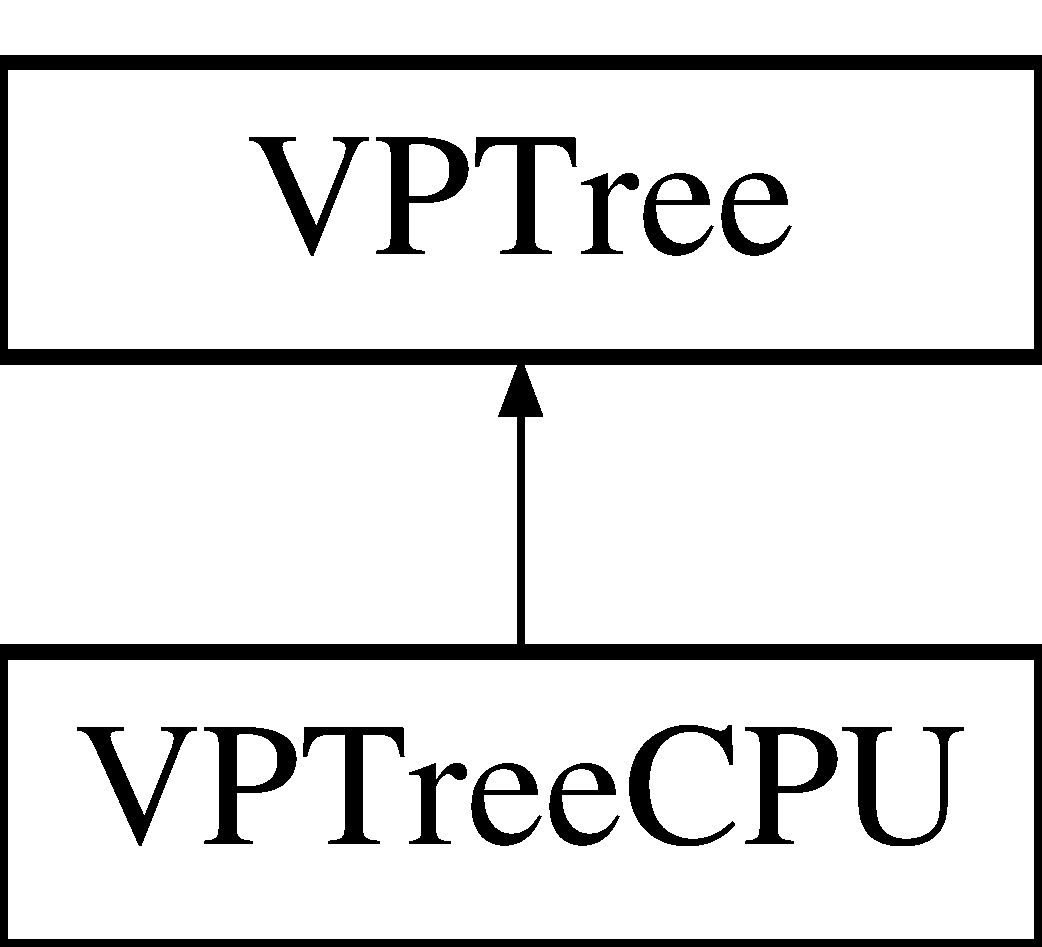
\includegraphics[height=2.000000cm]{classVPTree}
\end{center}
\end{figure}
\subsection*{Public Member Functions}
\begin{DoxyCompactItemize}
\item 
\hypertarget{classVPTree_aeac6b50747fdf3e85bf029460b6a1693}{}{\bfseries V\+P\+Tree} (const std\+::vector$<$ float $>$ \&data, int dim)\label{classVPTree_aeac6b50747fdf3e85bf029460b6a1693}

\end{DoxyCompactItemize}
\subsection*{Protected Attributes}
\begin{DoxyCompactItemize}
\item 
\hypertarget{classVPTree_ad6448be4cdc0e650706d1d99741b35c2}{}const std\+::vector$<$ float $>$ \& {\bfseries \+\_\+data}\label{classVPTree_ad6448be4cdc0e650706d1d99741b35c2}

\item 
\hypertarget{classVPTree_ac1aa451a8af463c442d3791d918bced6}{}int {\bfseries \+\_\+dim}\label{classVPTree_ac1aa451a8af463c442d3791d918bced6}

\end{DoxyCompactItemize}


The documentation for this class was generated from the following file\+:\begin{DoxyCompactItemize}
\item 
knn/vp\+\_\+tree.\+hpp\end{DoxyCompactItemize}

\hypertarget{classVPTreeCPU}{}\section{V\+P\+Tree\+C\+P\+U Class Reference}
\label{classVPTreeCPU}\index{V\+P\+Tree\+C\+P\+U@{V\+P\+Tree\+C\+P\+U}}
Inheritance diagram for V\+P\+Tree\+C\+P\+U\+:\begin{figure}[H]
\begin{center}
\leavevmode
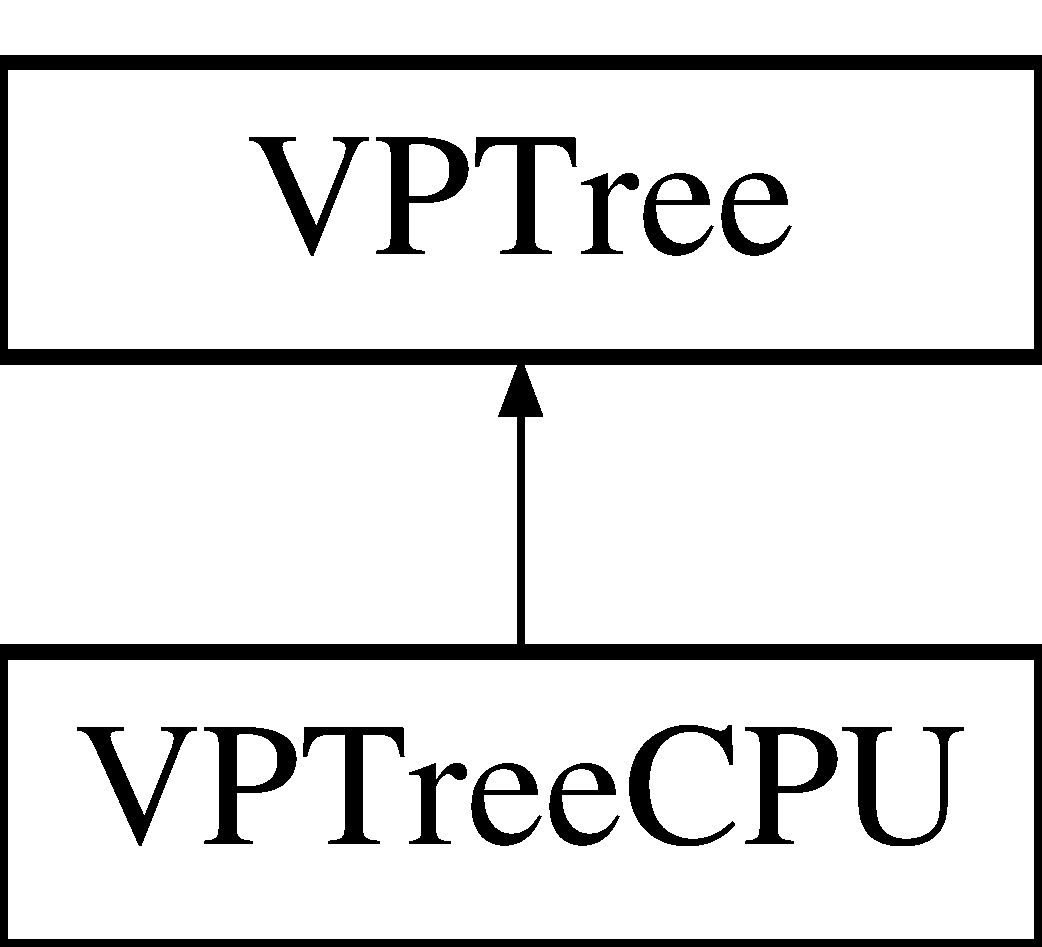
\includegraphics[height=2.000000cm]{classVPTreeCPU}
\end{center}
\end{figure}
\subsection*{Public Member Functions}
\begin{DoxyCompactItemize}
\item 
\hypertarget{classVPTreeCPU_ae657717bae418b4fb8980d06bc3408ce}{}{\bfseries V\+P\+Tree\+C\+P\+U} (const std\+::vector$<$ float $>$ \&data, int dim)\label{classVPTreeCPU_ae657717bae418b4fb8980d06bc3408ce}

\item 
virtual float \hyperlink{classVPTreeCPU_ab0a19f258e0ee042e7a244a2e2a06eb0}{dist2} (int a, int b)
\end{DoxyCompactItemize}
\subsection*{Protected Member Functions}
\begin{DoxyCompactItemize}
\item 
int \hyperlink{classVPTreeCPU_a5f1383c790fde3e76205d15d2948adca}{select\+\_\+vp} (const std\+::vector$<$ \hyperlink{classifloatn}{ifloat} $>$ \&index\+\_\+set)
\item 
int \hyperlink{classVPTreeCPU_a6b43ff7e4f9385c2674530a68b70f203}{make\+\_\+vp\+\_\+tree} (std\+::vector$<$ \hyperlink{classifloatn}{ifloat} $>$ \&index\+\_\+set)
\item 
void \hyperlink{classVPTreeCPU_a6ea3cda7de7a4d12ec453d22e6873a12}{dist2} (int p, std\+::vector$<$ \hyperlink{classifloatn}{ifloat} $>$ \&index\+\_\+set)
\item 
\hypertarget{classVPTreeCPU_a561eceaafc0efb117e432e7009ce0aab}{}void {\bfseries print\+\_\+tree} ()\label{classVPTreeCPU_a561eceaafc0efb117e432e7009ce0aab}

\end{DoxyCompactItemize}
\subsection*{Protected Attributes}
\begin{DoxyCompactItemize}
\item 
\hypertarget{classVPTreeCPU_ad8c9ea49deda6751e6b66e6f9c0ec8c2}{}std\+::vector$<$ \hyperlink{structvp__node__t}{vp\+\_\+node} $>$ {\bfseries \+\_\+tree}\label{classVPTreeCPU_ad8c9ea49deda6751e6b66e6f9c0ec8c2}

\end{DoxyCompactItemize}


\subsection{Member Function Documentation}
\hypertarget{classVPTreeCPU_ab0a19f258e0ee042e7a244a2e2a06eb0}{}\index{V\+P\+Tree\+C\+P\+U@{V\+P\+Tree\+C\+P\+U}!dist2@{dist2}}
\index{dist2@{dist2}!V\+P\+Tree\+C\+P\+U@{V\+P\+Tree\+C\+P\+U}}
\subsubsection[{dist2}]{\setlength{\rightskip}{0pt plus 5cm}float V\+P\+Tree\+C\+P\+U\+::dist2 (
\begin{DoxyParamCaption}
\item[{int}]{a, }
\item[{int}]{b}
\end{DoxyParamCaption}
)\hspace{0.3cm}{\ttfamily [inline]}, {\ttfamily [virtual]}}\label{classVPTreeCPU_ab0a19f258e0ee042e7a244a2e2a06eb0}
Distance function used for the metric space. You should override this function for having a default metric. \+: index of an element in the data array \+: index of an element in the data array \begin{DoxyReturn}{Returns}
\+: distance between element of index a and b 
\end{DoxyReturn}
\hypertarget{classVPTreeCPU_a6ea3cda7de7a4d12ec453d22e6873a12}{}\index{V\+P\+Tree\+C\+P\+U@{V\+P\+Tree\+C\+P\+U}!dist2@{dist2}}
\index{dist2@{dist2}!V\+P\+Tree\+C\+P\+U@{V\+P\+Tree\+C\+P\+U}}
\subsubsection[{dist2}]{\setlength{\rightskip}{0pt plus 5cm}void V\+P\+Tree\+C\+P\+U\+::dist2 (
\begin{DoxyParamCaption}
\item[{int}]{p, }
\item[{std\+::vector$<$ {\bf ifloat} $>$ \&}]{index\+\_\+set}
\end{DoxyParamCaption}
)\hspace{0.3cm}{\ttfamily [inline]}, {\ttfamily [protected]}}\label{classVPTreeCPU_a6ea3cda7de7a4d12ec453d22e6873a12}
Evaluates the distance between p and the set index\+\_\+set setting each float in index\+\_\+set \hypertarget{classVPTreeCPU_a6b43ff7e4f9385c2674530a68b70f203}{}\index{V\+P\+Tree\+C\+P\+U@{V\+P\+Tree\+C\+P\+U}!make\+\_\+vp\+\_\+tree@{make\+\_\+vp\+\_\+tree}}
\index{make\+\_\+vp\+\_\+tree@{make\+\_\+vp\+\_\+tree}!V\+P\+Tree\+C\+P\+U@{V\+P\+Tree\+C\+P\+U}}
\subsubsection[{make\+\_\+vp\+\_\+tree}]{\setlength{\rightskip}{0pt plus 5cm}int V\+P\+Tree\+C\+P\+U\+::make\+\_\+vp\+\_\+tree (
\begin{DoxyParamCaption}
\item[{std\+::vector$<$ {\bf ifloat} $>$ \&}]{index\+\_\+set}
\end{DoxyParamCaption}
)\hspace{0.3cm}{\ttfamily [inline]}, {\ttfamily [protected]}}\label{classVPTreeCPU_a6b43ff7e4f9385c2674530a68b70f203}
Constructs populating the \+\_\+tree vector a vp\+\_\+tree corresponding to the data stored in the \+\_\+data vector and specified in the index\+\_\+set \hypertarget{classVPTreeCPU_a5f1383c790fde3e76205d15d2948adca}{}\index{V\+P\+Tree\+C\+P\+U@{V\+P\+Tree\+C\+P\+U}!select\+\_\+vp@{select\+\_\+vp}}
\index{select\+\_\+vp@{select\+\_\+vp}!V\+P\+Tree\+C\+P\+U@{V\+P\+Tree\+C\+P\+U}}
\subsubsection[{select\+\_\+vp}]{\setlength{\rightskip}{0pt plus 5cm}int V\+P\+Tree\+C\+P\+U\+::select\+\_\+vp (
\begin{DoxyParamCaption}
\item[{const std\+::vector$<$ {\bf ifloat} $>$ \&}]{index\+\_\+set}
\end{DoxyParamCaption}
)\hspace{0.3cm}{\ttfamily [inline]}, {\ttfamily [protected]}}\label{classVPTreeCPU_a5f1383c790fde3e76205d15d2948adca}
Select among elements in index\+\_\+set the vantage point to split the Tree

Basic implementation still. Don\textquotesingle{}t see the point for a more complicated code 

The documentation for this class was generated from the following file\+:\begin{DoxyCompactItemize}
\item 
knn/vp\+\_\+tree\+\_\+cpu.\+hpp\end{DoxyCompactItemize}

%--- End generated contents ---

% Index
\backmatter
\newpage
\phantomsection
\clearemptydoublepage
\addcontentsline{toc}{chapter}{Index}
\printindex

\end{document}
